%%%%%%%%%%%%%%%%%%%%%%%%%%%%%%%%%%%%%%%%%%%%%%%%%%%%%%%%%%%%%%%%%%%%%%%%%%%%%%%%
%% Title (en): Multiagent Systems and Organizations                           %%
%% Title (cs): Multiagentní systémy a organizace                              %%
%%                                                                            %%
%% Author: Bc. Lukáš Kúdela                                                   %%
%% Supervisor: Prof. RNDr. Petr Štěpánek, DrSc.                               %%
%%                                                                            %%
%% Academic year: 2011/2012                                                   %%
%%%%%%%%%%%%%%%%%%%%%%%%%%%%%%%%%%%%%%%%%%%%%%%%%%%%%%%%%%%%%%%%%%%%%%%%%%%%%%%%

\chapter{Modelling Organizations -- Platform-Independent Metamodel -- Thespian}

In this chapter we will describe Thespian - our attempt at a platform independent metamodel (PIMM) for organization-centric multiagent systems (OCMASs).

% Platform-idenpendent model
In software engineering, \textit{platform-independent model} (PIM) is a model of a software system, that is independent of the specific technological platform used to implement it.
%\cite{Wikipedia-PlatformIndependentModel}
The main motivation to use a PIM is to build the model once and then automatically transform it to any number of platform-specific models (PSMs) for different (ALT: various) deployment platforms.

% Thespian name inspiration - Thespis of Icaria
Thespian is named after \textit{Thespis of Icaria} (present-day Dionysos, Greece), who lived in the 6th century BC and, according to certain Ancient Greece sources and especially Aristotle, was the first person ever to appear on stage as an actor playing a character in a play (instead of (ALT: as opposed to) speaking as himself) \cite{Wikipedia-Thespis}.

% Thespian inspiration - Aalaadin, O&P, PIM4Agents and powerJade
Thespian is inspired by all four metamodels introduced in the previous chapter: Aalaadin, O\&P, PIM4Agents and powerJade.
Similarly to Aalaadin, it contains both dynamic and static concepts (called \textit{core} and \textit{methodological} concepts in Aalaadin). Instances of dynamic/static concepts will end up as run-time/design-time entities in the platform-specific model.
Like O\&P, it can be used to model holonic MASes.
Similarly to PIM4Agents, it enables explicit modelling of protocol and messages exchanged in these protocols (ALT: in them). 
And finally like powerJade, it is able to represent competences (powers) and responsibilities (requirements) of roles.

% Two partitions: {organization, player and protocol}, {static and dynamic}
The Thespian metamodel can be partitioned in two orthogonal ways.
The first partition divides the concepts according to the area they represent: organization, player or protocol.
The second partition separates the concepts based on whether they are static (design-time) or dynamic (run-time) in nature.
Both partitions will be described in the following sections; the integrated metamodel will be presented in the last section.

%%%%%%%%%%%%%%%%%%%%%%%%%%%%%%%%%%%%%%%%%%%%%%%%%%%%%%%%%%%%%%%%%%%%%%%%%%%%%%%%
\section{Organization Metamodel}

% Organization metamodel - usage
The Organization metamodel (figure~\ref{figure:thespian-organization-metamodel}) contains concepts that represent organizations and roles with powers (ALT: competences) and requirements (ALT: responsibilities).

\subsection*{Organization and OrganizaitonClass}



\subsection*{Role and RoleInstance (Position)}

\subsection*{Power}

% Figure: Thespian organization metamodel
\begin{figure}[ht]
	\centering
	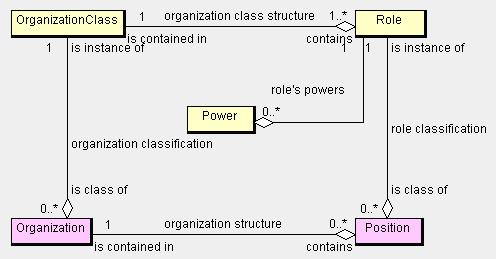
\includegraphics[width=\textwidth]{images/thespian-organization-metamodel.png}
	\caption{The Organization fragment of the Thespian metamodel}
	\label{figure:thespian-organization-metamodel}
\end{figure}

%%%%%%%%%%%%%%%%%%%%%%%%%%%%%%%%%%%%%%%%%%%%%%%%%%%%%%%%%%%%%%%%%%%%%%%%%%%%%%%%
\section{Player Metamodel}

% Player metamodel - usage
The Player metamodel (figure~\ref{figure:thespian-player-metamodel}) contains modelling constructs that can be used to model players and their abilities.

\subsection*{Player and PlayerClass}

\subsection*{Requirement}

% Figure: Thespian player metamodel
\begin{figure}[ht]
	\centering
	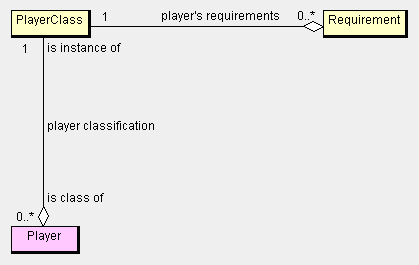
\includegraphics[width=\textwidth]{images/thespian-player-metamodel.png}
	\caption{The Player fragment of the Thespian metamodel}
	\label{figure:thespian-player-metamodel}
\end{figure}

%%%%%%%%%%%%%%%%%%%%%%%%%%%%%%%%%%%%%%%%%%%%%%%%%%%%%%%%%%%%%%%%%%%%%%%%%%%%%%%%
\section{Protocol Metamodel}

% Protocol metamodel - usage
The Protocol metamodel (figure~\ref{figure:thespian-protocol-metamodel}) contains abstractions that abstract model interaction protocols between a player and an organization or role and among roles themselves.

\subsection*{Protocol}

\subsection*{Party}

\subsection*{Message}

% Figure: Thespian protocol metamodel
\begin{figure}[ht]
	\centering
	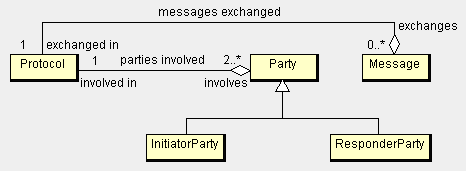
\includegraphics[width=\textwidth]{images/thespian-protocol-metamodel.png}
	\caption{The Protocol fragment of the Thespian metamodel}
	\label{figure:thespian-protocol-metamodel}
\end{figure}

%%%%%%%%%%%%%%%%%%%%%%%%%%%%%%%%%%%%%%%%%%%%%%%%%%%%%%%%%%%%%%%%%%%%%%%%%%%%%%%%
\section{Static (Design-Time) Metamodel}	

% Static metamodel - usage
The Static metamodel contains concepts that represent static entities - entities that are created/modified at design-time, i.e. in the MAS source code.

% Figure: Thespian static metamodel
\begin{figure}[ht]
	\centering
	
\includegraphics[width=\textwidth]{images/thespian-static-metamodel.png}
	\caption{The static fragment of the Thespian metamodel}
	\label{figure:thespian-static-metamodel}
\end{figure}

%%%%%%%%%%%%%%%%%%%%%%%%%%%%%%%%%%%%%%%%%%%%%%%%%%%%%%%%%%%%%%%%%%%%%%%%%%%%%%%%
\section{Dynamic (Run-Time) Metamodel}

% Dynamic metamodel - usage
The Dynamic metamodel contains abstractions that abstract dynamic entities - entities that are created/modified at run-rime, i.e. in the actual running MAS.

% Figure: Thespian dynamic metamodel
\begin{figure}[ht]
	\centering
	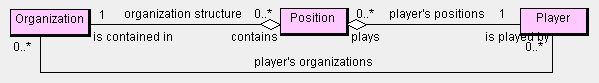
\includegraphics[width=\textwidth]{images/thespian-dynamic-metamodel.png}
	\caption{The dynamic fragment of the Thespian metamodel}
	\label{figure:thespian-dynamic-metamodel}
\end{figure}

%%%%%%%%%%%%%%%%%%%%%%%%%%%%%%%%%%%%%%%%%%%%%%%%%%%%%%%%%%%%%%%%%%%%%%%%%%%%%%%%
\section{Integrated Metamodel}

Figure~\ref{figure:thespian-integrated-metamodel} show the integrated Thespian metamodel.

\subsection*{Association between Player and Position}

\subsection*{Association between Player and Organization}

\subsection*{Association between OrganizationClass and Party}

\subsection*{Associaiton between RoleClass and Party}

\subsection*{Association between PlayerClass and Party}

% Figure: Thespian integrated metamodel
\begin{figure}[ht]
	\centering
	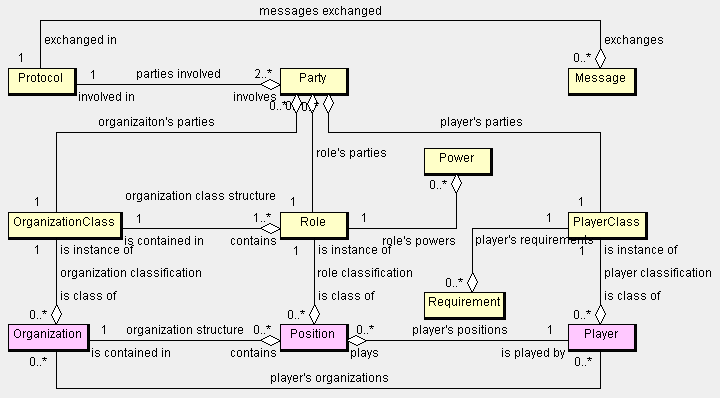
\includegraphics[width=\textwidth]{images/thespian-integrated-metamodel.png}
	\caption{The integrated Thespian metamodel}
	\label{figure:thespian-integrated-metamodel}
\end{figure}

